% Created by tikzDevice version 0.12.3.1 on 2022-03-16 15:46:07
% !TEX encoding = UTF-8 Unicode
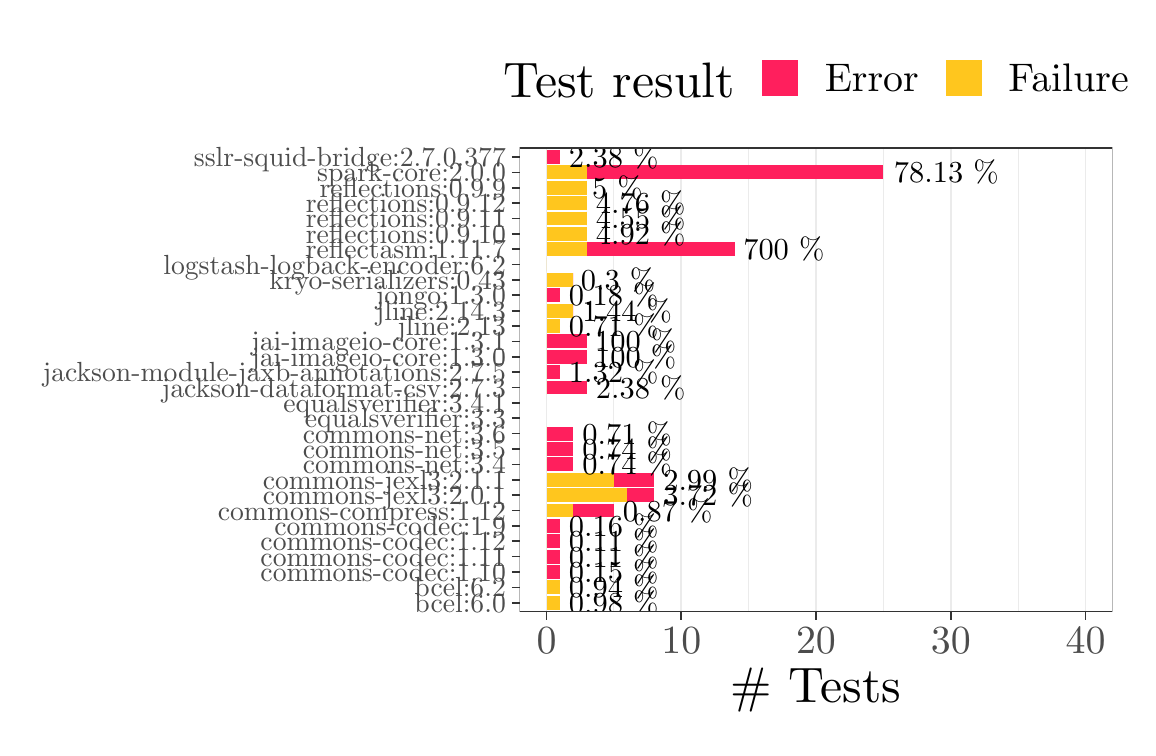
\begin{tikzpicture}[x=1pt,y=1pt]
\definecolor{fillColor}{RGB}{255,255,255}
\path[use as bounding box,fill=fillColor,fill opacity=0.00] (0,0) rectangle (397.48,252.94);
\begin{scope}
\path[clip] (  0.00,  0.00) rectangle (397.48,252.94);
\definecolor{drawColor}{RGB}{255,255,255}
\definecolor{fillColor}{RGB}{255,255,255}

\path[draw=drawColor,line width= 0.6pt,line join=round,line cap=round,fill=fillColor] (  0.00,  0.00) rectangle (397.48,252.94);
\end{scope}
\begin{scope}
\path[clip] (177.74, 41.81) rectangle (391.98,209.55);
\definecolor{fillColor}{RGB}{255,255,255}

\path[fill=fillColor] (177.74, 41.81) rectangle (391.98,209.55);
\definecolor{drawColor}{gray}{0.92}

\path[draw=drawColor,line width= 0.3pt,line join=round] (211.83, 41.81) --
	(211.83,209.55);

\path[draw=drawColor,line width= 0.3pt,line join=round] (260.52, 41.81) --
	(260.52,209.55);

\path[draw=drawColor,line width= 0.3pt,line join=round] (309.21, 41.81) --
	(309.21,209.55);

\path[draw=drawColor,line width= 0.3pt,line join=round] (357.90, 41.81) --
	(357.90,209.55);

\path[draw=drawColor,line width= 0.6pt,line join=round] (187.48, 41.81) --
	(187.48,209.55);

\path[draw=drawColor,line width= 0.6pt,line join=round] (236.17, 41.81) --
	(236.17,209.55);

\path[draw=drawColor,line width= 0.6pt,line join=round] (284.86, 41.81) --
	(284.86,209.55);

\path[draw=drawColor,line width= 0.6pt,line join=round] (333.56, 41.81) --
	(333.56,209.55);

\path[draw=drawColor,line width= 0.6pt,line join=round] (382.25, 41.81) --
	(382.25,209.55);
\definecolor{fillColor}{RGB}{255,31,93}

\path[fill=fillColor] (192.35, 42.65) rectangle (192.35, 47.64);

\path[fill=fillColor] (192.35, 48.20) rectangle (192.35, 53.20);

\path[fill=fillColor] (187.48, 53.75) rectangle (192.35, 58.75);

\path[fill=fillColor] (187.48, 59.31) rectangle (192.35, 64.31);

\path[fill=fillColor] (187.48, 64.86) rectangle (192.35, 69.86);

\path[fill=fillColor] (187.48, 70.42) rectangle (192.35, 75.42);

\path[fill=fillColor] (197.22, 75.97) rectangle (211.83, 80.97);

\path[fill=fillColor] (216.70, 81.53) rectangle (226.43, 86.52);

\path[fill=fillColor] (211.83, 87.08) rectangle (226.43, 92.08);

\path[fill=fillColor] (187.48, 92.63) rectangle (197.22, 97.63);

\path[fill=fillColor] (187.48, 98.19) rectangle (197.22,103.19);

\path[fill=fillColor] (187.48,103.74) rectangle (197.22,108.74);

\path[fill=fillColor] (187.48,120.40) rectangle (202.09,125.40);

\path[fill=fillColor] (187.48,125.96) rectangle (192.35,130.96);

\path[fill=fillColor] (187.48,131.51) rectangle (202.09,136.51);

\path[fill=fillColor] (187.48,137.07) rectangle (202.09,142.07);

\path[fill=fillColor] (192.35,142.62) rectangle (192.35,147.62);

\path[fill=fillColor] (197.22,148.18) rectangle (197.22,153.17);

\path[fill=fillColor] (187.48,153.73) rectangle (192.35,158.73);

\path[fill=fillColor] (197.22,159.28) rectangle (197.22,164.28);

\path[fill=fillColor] (202.09,170.39) rectangle (255.65,175.39);

\path[fill=fillColor] (202.09,175.95) rectangle (202.09,180.94);

\path[fill=fillColor] (202.09,181.50) rectangle (202.09,186.50);

\path[fill=fillColor] (202.09,187.05) rectangle (202.09,192.05);

\path[fill=fillColor] (202.09,192.61) rectangle (202.09,197.61);

\path[fill=fillColor] (202.09,198.16) rectangle (309.21,203.16);

\path[fill=fillColor] (187.48,203.72) rectangle (192.35,208.72);
\definecolor{fillColor}{RGB}{255,198,30}

\path[fill=fillColor] (187.48, 42.65) rectangle (192.35, 47.64);

\path[fill=fillColor] (187.48, 48.20) rectangle (192.35, 53.20);

\path[fill=fillColor] (187.48, 53.75) rectangle (187.48, 58.75);

\path[fill=fillColor] (187.48, 59.31) rectangle (187.48, 64.31);

\path[fill=fillColor] (187.48, 64.86) rectangle (187.48, 69.86);

\path[fill=fillColor] (187.48, 70.42) rectangle (187.48, 75.42);

\path[fill=fillColor] (187.48, 75.97) rectangle (197.22, 80.97);

\path[fill=fillColor] (187.48, 81.53) rectangle (216.70, 86.52);

\path[fill=fillColor] (187.48, 87.08) rectangle (211.83, 92.08);

\path[fill=fillColor] (187.48, 92.63) rectangle (187.48, 97.63);

\path[fill=fillColor] (187.48, 98.19) rectangle (187.48,103.19);

\path[fill=fillColor] (187.48,103.74) rectangle (187.48,108.74);

\path[fill=fillColor] (187.48,120.40) rectangle (187.48,125.40);

\path[fill=fillColor] (187.48,125.96) rectangle (187.48,130.96);

\path[fill=fillColor] (187.48,131.51) rectangle (187.48,136.51);

\path[fill=fillColor] (187.48,137.07) rectangle (187.48,142.07);

\path[fill=fillColor] (187.48,142.62) rectangle (192.35,147.62);

\path[fill=fillColor] (187.48,148.18) rectangle (197.22,153.17);

\path[fill=fillColor] (187.48,153.73) rectangle (187.48,158.73);

\path[fill=fillColor] (187.48,159.28) rectangle (197.22,164.28);

\path[fill=fillColor] (187.48,164.84) rectangle (187.48,169.84);

\path[fill=fillColor] (187.48,170.39) rectangle (202.09,175.39);

\path[fill=fillColor] (187.48,175.95) rectangle (202.09,180.94);

\path[fill=fillColor] (187.48,181.50) rectangle (202.09,186.50);

\path[fill=fillColor] (187.48,187.05) rectangle (202.09,192.05);

\path[fill=fillColor] (187.48,192.61) rectangle (202.09,197.61);

\path[fill=fillColor] (187.48,198.16) rectangle (202.09,203.16);

\path[fill=fillColor] (187.48,203.72) rectangle (187.48,208.72);
\definecolor{drawColor}{RGB}{0,0,0}

\node[text=drawColor,anchor=base west,inner sep=0pt, outer sep=0pt, scale=  1.10] at (258.59,169.09) {700 \%};

\node[text=drawColor,anchor=base west,inner sep=0pt, outer sep=0pt, scale=  1.10] at (205.34,119.10) {2.38 \%};

\node[text=drawColor,anchor=base west,inner sep=0pt, outer sep=0pt, scale=  1.10] at (195.60,124.66) {1.32 \%};

\node[text=drawColor,anchor=base west,inner sep=0pt, outer sep=0pt, scale=  1.10] at (200.47,102.44) {0.71 \%};

\node[text=drawColor,anchor=base west,inner sep=0pt, outer sep=0pt, scale=  1.10] at (200.47, 91.33) {0.74 \%};

\node[text=drawColor,anchor=base west,inner sep=0pt, outer sep=0pt, scale=  1.10] at (200.47, 96.89) {0.74 \%};

\node[text=drawColor,anchor=base west,inner sep=0pt, outer sep=0pt, scale=  1.10] at (195.60,202.41) {2.38 \%};

\node[text=drawColor,anchor=base west,inner sep=0pt, outer sep=0pt, scale=  1.10] at (195.60, 41.34) {0.98 \%};

\node[text=drawColor,anchor=base west,inner sep=0pt, outer sep=0pt, scale=  1.10] at (195.60, 46.90) {0.94 \%};

\node[text=drawColor,anchor=base west,inner sep=0pt, outer sep=0pt, scale=  1.10] at (195.60, 52.45) {0.15 \%};

\node[text=drawColor,anchor=base west,inner sep=0pt, outer sep=0pt, scale=  1.10] at (195.60, 63.56) {0.11 \%};

\node[text=drawColor,anchor=base west,inner sep=0pt, outer sep=0pt, scale=  1.10] at (195.60, 69.11) {0.16 \%};

\node[text=drawColor,anchor=base west,inner sep=0pt, outer sep=0pt, scale=  1.10] at (195.60, 58.01) {0.11 \%};

\node[text=drawColor,anchor=base west,inner sep=0pt, outer sep=0pt, scale=  1.10] at (215.08, 74.67) {0.87 \%};

\node[text=drawColor,anchor=base west,inner sep=0pt, outer sep=0pt, scale=  1.10] at (229.68, 85.78) {2.99 \%};

\node[text=drawColor,anchor=base west,inner sep=0pt, outer sep=0pt, scale=  1.10] at (229.68, 80.22) {3.72 \%};

\node[text=drawColor,anchor=base west,inner sep=0pt, outer sep=0pt, scale=  1.10] at (195.60,152.43) {0.18 \%};

\node[text=drawColor,anchor=base west,inner sep=0pt, outer sep=0pt, scale=  1.10] at (195.60,141.32) {0.71 \%};

\node[text=drawColor,anchor=base west,inner sep=0pt, outer sep=0pt, scale=  1.10] at (200.47,146.87) {1.44 \%};

\node[text=drawColor,anchor=base west,inner sep=0pt, outer sep=0pt, scale=  1.10] at (205.03,135.76) {100 \%};

\node[text=drawColor,anchor=base west,inner sep=0pt, outer sep=0pt, scale=  1.10] at (205.03,130.21) {100 \%};

\node[text=drawColor,anchor=base west,inner sep=0pt, outer sep=0pt, scale=  1.10] at (199.92,157.98) {0.3 \%};

\node[text=drawColor,anchor=base west,inner sep=0pt, outer sep=0pt, scale=  1.10] at (313.01,196.86) {78.13 \%};

\node[text=drawColor,anchor=base west,inner sep=0pt, outer sep=0pt, scale=  1.10] at (205.34,174.64) {4.92 \%};

\node[text=drawColor,anchor=base west,inner sep=0pt, outer sep=0pt, scale=  1.10] at (205.34,180.20) {4.55 \%};

\node[text=drawColor,anchor=base west,inner sep=0pt, outer sep=0pt, scale=  1.10] at (203.93,191.31) {5 \%};

\node[text=drawColor,anchor=base west,inner sep=0pt, outer sep=0pt, scale=  1.10] at (205.34,185.75) {4.76 \%};
\definecolor{drawColor}{gray}{0.20}

\path[draw=drawColor,line width= 0.6pt,line join=round,line cap=round] (177.74, 41.81) rectangle (391.98,209.55);
\end{scope}
\begin{scope}
\path[clip] (  0.00,  0.00) rectangle (397.48,252.94);
\definecolor{drawColor}{gray}{0.30}

\node[text=drawColor,anchor=base east,inner sep=0pt, outer sep=0pt, scale=  1.00] at (172.79, 41.70) {bcel:6.0};

\node[text=drawColor,anchor=base east,inner sep=0pt, outer sep=0pt, scale=  1.00] at (172.79, 47.26) {bcel:6.2};

\node[text=drawColor,anchor=base east,inner sep=0pt, outer sep=0pt, scale=  1.00] at (172.79, 52.81) {commons-codec:1.10};

\node[text=drawColor,anchor=base east,inner sep=0pt, outer sep=0pt, scale=  1.00] at (172.79, 58.36) {commons-codec:1.11};

\node[text=drawColor,anchor=base east,inner sep=0pt, outer sep=0pt, scale=  1.00] at (172.79, 63.92) {commons-codec:1.12};

\node[text=drawColor,anchor=base east,inner sep=0pt, outer sep=0pt, scale=  1.00] at (172.79, 69.47) {commons-codec:1.9};

\node[text=drawColor,anchor=base east,inner sep=0pt, outer sep=0pt, scale=  1.00] at (172.79, 75.03) {commons-compress:1.12};

\node[text=drawColor,anchor=base east,inner sep=0pt, outer sep=0pt, scale=  1.00] at (172.79, 80.58) {commons-jexl3:2.0.1};

\node[text=drawColor,anchor=base east,inner sep=0pt, outer sep=0pt, scale=  1.00] at (172.79, 86.14) {commons-jexl3:2.1.1};

\node[text=drawColor,anchor=base east,inner sep=0pt, outer sep=0pt, scale=  1.00] at (172.79, 91.69) {commons-net:3.4};

\node[text=drawColor,anchor=base east,inner sep=0pt, outer sep=0pt, scale=  1.00] at (172.79, 97.24) {commons-net:3.5};

\node[text=drawColor,anchor=base east,inner sep=0pt, outer sep=0pt, scale=  1.00] at (172.79,102.80) {commons-net:3.6};

\node[text=drawColor,anchor=base east,inner sep=0pt, outer sep=0pt, scale=  1.00] at (172.79,108.35) {equalsverifier:3.3};

\node[text=drawColor,anchor=base east,inner sep=0pt, outer sep=0pt, scale=  1.00] at (172.79,113.91) {equalsverifier:3.4.1};

\node[text=drawColor,anchor=base east,inner sep=0pt, outer sep=0pt, scale=  1.00] at (172.79,119.46) {jackson-dataformat-csv:2.7.3};

\node[text=drawColor,anchor=base east,inner sep=0pt, outer sep=0pt, scale=  1.00] at (172.79,125.01) {jackson-module-jaxb-annotations:2.7.5};

\node[text=drawColor,anchor=base east,inner sep=0pt, outer sep=0pt, scale=  1.00] at (172.79,130.57) {jai-imageio-core:1.3.0};

\node[text=drawColor,anchor=base east,inner sep=0pt, outer sep=0pt, scale=  1.00] at (172.79,136.12) {jai-imageio-core:1.3.1};

\node[text=drawColor,anchor=base east,inner sep=0pt, outer sep=0pt, scale=  1.00] at (172.79,141.68) {jline:2.13};

\node[text=drawColor,anchor=base east,inner sep=0pt, outer sep=0pt, scale=  1.00] at (172.79,147.23) {jline:2.14.3};

\node[text=drawColor,anchor=base east,inner sep=0pt, outer sep=0pt, scale=  1.00] at (172.79,152.79) {jongo:1.3.0};

\node[text=drawColor,anchor=base east,inner sep=0pt, outer sep=0pt, scale=  1.00] at (172.79,158.34) {kryo-serializers:0.43};

\node[text=drawColor,anchor=base east,inner sep=0pt, outer sep=0pt, scale=  1.00] at (172.79,163.89) {logstash-logback-encoder:6.2};

\node[text=drawColor,anchor=base east,inner sep=0pt, outer sep=0pt, scale=  1.00] at (172.79,169.45) {reflectasm:1.11.7};

\node[text=drawColor,anchor=base east,inner sep=0pt, outer sep=0pt, scale=  1.00] at (172.79,175.00) {reflections:0.9.10};

\node[text=drawColor,anchor=base east,inner sep=0pt, outer sep=0pt, scale=  1.00] at (172.79,180.56) {reflections:0.9.11};

\node[text=drawColor,anchor=base east,inner sep=0pt, outer sep=0pt, scale=  1.00] at (172.79,186.11) {reflections:0.9.12};

\node[text=drawColor,anchor=base east,inner sep=0pt, outer sep=0pt, scale=  1.00] at (172.79,191.66) {reflections:0.9.9};

\node[text=drawColor,anchor=base east,inner sep=0pt, outer sep=0pt, scale=  1.00] at (172.79,197.22) {spark-core:2.0.0};

\node[text=drawColor,anchor=base east,inner sep=0pt, outer sep=0pt, scale=  1.00] at (172.79,202.77) {sslr-squid-bridge:2.7.0.377};
\end{scope}
\begin{scope}
\path[clip] (  0.00,  0.00) rectangle (397.48,252.94);
\definecolor{drawColor}{gray}{0.20}

\path[draw=drawColor,line width= 0.6pt,line join=round] (174.99, 45.15) --
	(177.74, 45.15);

\path[draw=drawColor,line width= 0.6pt,line join=round] (174.99, 50.70) --
	(177.74, 50.70);

\path[draw=drawColor,line width= 0.6pt,line join=round] (174.99, 56.25) --
	(177.74, 56.25);

\path[draw=drawColor,line width= 0.6pt,line join=round] (174.99, 61.81) --
	(177.74, 61.81);

\path[draw=drawColor,line width= 0.6pt,line join=round] (174.99, 67.36) --
	(177.74, 67.36);

\path[draw=drawColor,line width= 0.6pt,line join=round] (174.99, 72.92) --
	(177.74, 72.92);

\path[draw=drawColor,line width= 0.6pt,line join=round] (174.99, 78.47) --
	(177.74, 78.47);

\path[draw=drawColor,line width= 0.6pt,line join=round] (174.99, 84.02) --
	(177.74, 84.02);

\path[draw=drawColor,line width= 0.6pt,line join=round] (174.99, 89.58) --
	(177.74, 89.58);

\path[draw=drawColor,line width= 0.6pt,line join=round] (174.99, 95.13) --
	(177.74, 95.13);

\path[draw=drawColor,line width= 0.6pt,line join=round] (174.99,100.69) --
	(177.74,100.69);

\path[draw=drawColor,line width= 0.6pt,line join=round] (174.99,106.24) --
	(177.74,106.24);

\path[draw=drawColor,line width= 0.6pt,line join=round] (174.99,111.80) --
	(177.74,111.80);

\path[draw=drawColor,line width= 0.6pt,line join=round] (174.99,117.35) --
	(177.74,117.35);

\path[draw=drawColor,line width= 0.6pt,line join=round] (174.99,122.90) --
	(177.74,122.90);

\path[draw=drawColor,line width= 0.6pt,line join=round] (174.99,128.46) --
	(177.74,128.46);

\path[draw=drawColor,line width= 0.6pt,line join=round] (174.99,134.01) --
	(177.74,134.01);

\path[draw=drawColor,line width= 0.6pt,line join=round] (174.99,139.57) --
	(177.74,139.57);

\path[draw=drawColor,line width= 0.6pt,line join=round] (174.99,145.12) --
	(177.74,145.12);

\path[draw=drawColor,line width= 0.6pt,line join=round] (174.99,150.67) --
	(177.74,150.67);

\path[draw=drawColor,line width= 0.6pt,line join=round] (174.99,156.23) --
	(177.74,156.23);

\path[draw=drawColor,line width= 0.6pt,line join=round] (174.99,161.78) --
	(177.74,161.78);

\path[draw=drawColor,line width= 0.6pt,line join=round] (174.99,167.34) --
	(177.74,167.34);

\path[draw=drawColor,line width= 0.6pt,line join=round] (174.99,172.89) --
	(177.74,172.89);

\path[draw=drawColor,line width= 0.6pt,line join=round] (174.99,178.45) --
	(177.74,178.45);

\path[draw=drawColor,line width= 0.6pt,line join=round] (174.99,184.00) --
	(177.74,184.00);

\path[draw=drawColor,line width= 0.6pt,line join=round] (174.99,189.55) --
	(177.74,189.55);

\path[draw=drawColor,line width= 0.6pt,line join=round] (174.99,195.11) --
	(177.74,195.11);

\path[draw=drawColor,line width= 0.6pt,line join=round] (174.99,200.66) --
	(177.74,200.66);

\path[draw=drawColor,line width= 0.6pt,line join=round] (174.99,206.22) --
	(177.74,206.22);
\end{scope}
\begin{scope}
\path[clip] (  0.00,  0.00) rectangle (397.48,252.94);
\definecolor{drawColor}{gray}{0.20}

\path[draw=drawColor,line width= 0.6pt,line join=round] (187.48, 39.06) --
	(187.48, 41.81);

\path[draw=drawColor,line width= 0.6pt,line join=round] (236.17, 39.06) --
	(236.17, 41.81);

\path[draw=drawColor,line width= 0.6pt,line join=round] (284.86, 39.06) --
	(284.86, 41.81);

\path[draw=drawColor,line width= 0.6pt,line join=round] (333.56, 39.06) --
	(333.56, 41.81);

\path[draw=drawColor,line width= 0.6pt,line join=round] (382.25, 39.06) --
	(382.25, 41.81);
\end{scope}
\begin{scope}
\path[clip] (  0.00,  0.00) rectangle (397.48,252.94);
\definecolor{drawColor}{gray}{0.30}

\node[text=drawColor,anchor=base,inner sep=0pt, outer sep=0pt, scale=  1.44] at (187.48, 26.95) {0};

\node[text=drawColor,anchor=base,inner sep=0pt, outer sep=0pt, scale=  1.44] at (236.17, 26.95) {10};

\node[text=drawColor,anchor=base,inner sep=0pt, outer sep=0pt, scale=  1.44] at (284.86, 26.95) {20};

\node[text=drawColor,anchor=base,inner sep=0pt, outer sep=0pt, scale=  1.44] at (333.56, 26.95) {30};

\node[text=drawColor,anchor=base,inner sep=0pt, outer sep=0pt, scale=  1.44] at (382.25, 26.95) {40};
\end{scope}
\begin{scope}
\path[clip] (  0.00,  0.00) rectangle (397.48,252.94);
\definecolor{drawColor}{RGB}{0,0,0}

\node[text=drawColor,anchor=base,inner sep=0pt, outer sep=0pt, scale=  1.80] at (284.86,  9.00) {\# Tests};
\end{scope}
\begin{scope}
\path[clip] (  0.00,  0.00) rectangle (397.48,252.94);
\definecolor{fillColor}{RGB}{255,255,255}

\path[fill=fillColor] (166.37,220.55) rectangle (403.35,247.45);
\end{scope}
\begin{scope}
\path[clip] (  0.00,  0.00) rectangle (397.48,252.94);
\definecolor{drawColor}{RGB}{0,0,0}

\node[text=drawColor,anchor=base west,inner sep=0pt, outer sep=0pt, scale=  1.80] at (171.87,227.80) {Test result};
\end{scope}
\begin{scope}
\path[clip] (  0.00,  0.00) rectangle (397.48,252.94);
\definecolor{fillColor}{RGB}{255,255,255}

\path[fill=fillColor] (264.60,227.49) rectangle (279.06,241.95);
\end{scope}
\begin{scope}
\path[clip] (  0.00,  0.00) rectangle (397.48,252.94);
\definecolor{fillColor}{RGB}{255,31,93}

\path[fill=fillColor] (265.32,228.20) rectangle (278.35,241.23);
\end{scope}
\begin{scope}
\path[clip] (  0.00,  0.00) rectangle (397.48,252.94);
\definecolor{fillColor}{RGB}{255,255,255}

\path[fill=fillColor] (330.97,227.49) rectangle (345.42,241.95);
\end{scope}
\begin{scope}
\path[clip] (  0.00,  0.00) rectangle (397.48,252.94);
\definecolor{fillColor}{RGB}{255,198,30}

\path[fill=fillColor] (331.68,228.20) rectangle (344.71,241.23);
\end{scope}
\begin{scope}
\path[clip] (  0.00,  0.00) rectangle (397.48,252.94);
\definecolor{drawColor}{RGB}{0,0,0}

\node[text=drawColor,anchor=base west,inner sep=0pt, outer sep=0pt, scale=  1.44] at (288.06,229.76) {Error};
\end{scope}
\begin{scope}
\path[clip] (  0.00,  0.00) rectangle (397.48,252.94);
\definecolor{drawColor}{RGB}{0,0,0}

\node[text=drawColor,anchor=base west,inner sep=0pt, outer sep=0pt, scale=  1.44] at (354.42,229.76) {Failure};
\end{scope}
\end{tikzpicture}
